\documentclass[16pt]{article}
\usepackage[utf8]{inputenc, lscape}
\usepackage[demo]{graphicx}
\usepackage[a4paper,bindingoffset=0.2in,%
            left=1.1in,right=0.85in,top=1in,bottom=1in,%
            footskip=.25in]{geometry}

\begin{document}

% data is from the presentation "cis_prel_pres" 3 days ago (levels) and 
% the scripts "i6_d25_6m_", "i6_d24_csd".

\newgeometry{left=1.5cm, right=1cm, top=3cm, bottom=1.5cm}

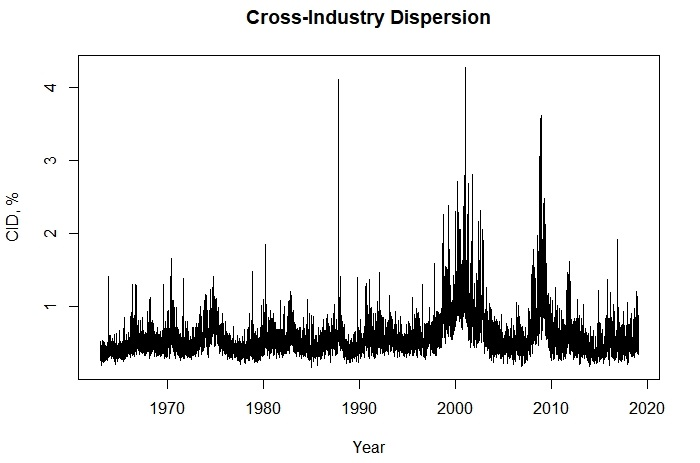
\includegraphics[width=1\textwidth]{ts_cid_00.jpeg}

\newpage

{\textbf{Results in levels:}}

\begin{table}[!htbp] \centering 
  \caption{Excess returns of decile $\beta_{CID}$-sorted portfolios} 
  \label{} 
  
\begin{tabular}{@{\extracolsep{-6pt}} cccccccccccc} 
\\[-1.8ex]\hline 
\hline \\[-1.8ex] 
 & D1 & D2 & D3 & D4 & D5 & D6 & D7 & D8 & D9 & D10 & LS(annualized) \\ 
\hline \\[-1.8ex] 
Mean ew & $0.069$ & $0.052$ & $0.047$ & $0.047$ & $0.044$ & $0.043$ & $0.045$ & $0.042$ & $0.039$ & $0.034$ & $$-$8.828$ \\ 
T\_stat & $7.800$ & $7.044$ & $6.682$ & $6.682$ & $6.221$ & $5.774$ & $5.810$ & $5.133$ & $4.345$ & $3.172$ & $$-$5.021$ \\ 
Mean vw & $0.037$ & $0.027$ & $0.031$ & $0.030$ & $0.026$ & $0.029$ & $0.029$ & $0.022$ & $0.019$ & $0.009$ & $$-$7.215$ \\ 
T\_stat & $3.391$ & $2.949$ & $3.624$ & $3.685$ & $3.253$ & $3.532$ & $3.438$ & $2.428$ & $1.894$ & $0.669$ & $$-$2.733$ \\ 
\hline \\[-1.8ex] 
\end{tabular} 
\end{table}


% Table created by stargazer v.5.2.2 by Marek Hlavac, Harvard University. E-mail: hlavac at fas.harvard.edu
% Date and time: Sun, Aug 18, 2019 - 5:07:25 PM
\begin{table}[!htbp] \centering 
  \caption{Abnormal returns of value-weighted long/short portfolios} 
  \label{} 
\begin{tabular}{@{\extracolsep{5pt}} ccccc} 
\\[-1.8ex]\hline 
\hline \\[-1.8ex] 
Statistic & Ret & Alpha CAPM & Alpha FF3 & Alpha FF5 \\ 
\hline \\[-1.8ex] 
Return & -7.308 & -8.316 & -11.088 & -10.332 \\ 
T-stat & [ -2.730] & [ -3.216] & [ -4.516] & [ -4.165] \\ 
\hline \\[-1.8ex] 
\end{tabular} 
\end{table}



% Table created by stargazer v.5.2.2 by Marek Hlavac, Harvard University. E-mail: hlavac at fas.harvard.edu
% Date and time: Sun, Aug 18, 2019 - 5:11:11 PM
\begin{table}[!htbp] \centering 
  \caption{Factor loadings} 
  \label{} 
\begin{tabular}{@{\extracolsep{-3pt}} ccccccccc} 
\\[-1.8ex]\hline 
\hline \\[-1.8ex] 
Ntile & Ret & Alpha & EMKT & HML & SMB & RMW & CMA & adjR2 \\ 
\hline \\[-1.8ex] 
1 & 0.037 & 0.016 & 1.063 & -0.192 & 0.407 & -0.219 & -0.174 & 0.757 \\ 
 & [ 3.371] & [ 2.994] & [ 172.759] & [ -14.774] & [ 36.783] & [ -13.702] & [ -9.235] &  \\ 
2 & 0.027 & 0.004 & 0.969 & -0.093 & 0.249 & -0.010 & -0.038 & 0.800 \\ 
 & [ 2.929] & [ 0.884] & [ 207.352] & [ -9.440] & [ 29.632] & [ -0.852] & [ -2.660] &  \\ 
3 & 0.031 & 0.008 & 0.927 & -0.084 & 0.155 & 0.014 & 0.038 & 0.829 \\ 
 & [ 3.598] & [ 2.165] & [ 231.465] & [ -9.884] & [ 21.514] & [ 1.352] & [ 3.066] &  \\ 
4 & 0.030 & 0.005 & 0.928 & -0.060 & 0.105 & 0.077 & 0.119 & 0.855 \\ 
 & [ 3.662] & [ 1.666] & [ 260.242] & [ -7.961] & [ 16.358] & [ 8.291] & [ 10.888] &  \\ 
5 & 0.026 & -0.001 & 0.932 & 0.005 & 0.083 & 0.129 & 0.126 & 0.874 \\ 
 & [ 3.229] & [ -0.189] & [ 285.878] & [ 0.681] & [ 14.143] & [ 15.209] & [ 12.638] &  \\ 
6 & 0.029 & 0.001 & 0.952 & 0.045 & 0.048 & 0.140 & 0.127 & 0.890 \\ 
 & [ 3.514] & [ 0.387] & [ 308.445] & [ 6.953] & [ 8.634] & [ 17.426] & [ 13.438] &  \\ 
7 & 0.029 & 0.000 & 0.983 & 0.106 & 0.019 & 0.147 & 0.094 & 0.891 \\ 
 & [ 3.419] & [ 0.030] & [ 309.228] & [ 15.803] & [ 3.252] & [ 17.753] & [ 9.717] &  \\ 
8 & 0.022 & -0.008 & 1.041 & 0.197 & 0.003 & 0.107 & 0.037 & 0.883 \\ 
 & [ 2.406] & [ -2.743] & [ 296.741] & [ 26.509] & [ 0.499] & [ 11.716] & [ 3.483] &  \\ 
9 & 0.019 & -0.015 & 1.125 & 0.402 & 0.037 & 0.111 & -0.145 & 0.855 \\ 
 & [ 1.879] & [ -3.788] & [ 258.997] & [ 43.741] & [ 4.757] & [ 9.814] & [ -10.928] &  \\ 
10 & 0.008 & -0.025 & 1.284 & 0.700 & 0.130 & -0.172 & -0.591 & 0.776 \\ 
 & [ 0.655] & [ -4.068] & [ 187.207] & [ 48.206] & [ 10.565] & [ -9.634] & [ -28.204] &  \\ 
LS & -0.029 & -0.041 & 0.221 & 0.892 & -0.277 & 0.047 & -0.418 & 0.130 \\ 
 & [ -2.730] & [ -4.165] & [ 19.834] & [ 37.894] & [ -13.838] & [ 1.642] & [ -12.279] &  \\ 
\hline \\[-1.8ex] 
\end{tabular} 
\end{table}



\begin{table}[!htbp] \centering 
  \caption{Fama-MacBeth egression of excess returns on characteristics} 
  \label{} 
\begin{tabular}{@{\extracolsep{5pt}} ccccc} 
\\[-1.8ex]\hline 
\hline \\[-1.8ex] 
 & Intercept & beta\_cimad & beta & size \\ 
\hline \\[-1.8ex] 
coefmean & $0.2278$ & $$-$0.0069$ & $0.0095$ & $$-$0.0165$ \\ 
se & $0.0132$ & $0.0013$ & $0.0080$ & $0.0011$ \\ 
tstat & $17.2100$ & $$-$5.1390$ & $1.1860$ & $$-$15.7000$ \\ 
r2 & $0.0215$ & $0.0215$ & $0.0215$ & $0.0215$ \\ 
\hline \\[-1.8ex] 
\end{tabular} 
\end{table}


\newpage

{\textbf{Results in differences:}}

% Table created by stargazer v.5.2.2 by Marek Hlavac, Harvard University. E-mail: hlavac at fas.harvard.edu
% Date and time: Thu, Aug 22, 2019 - 10:08:51 AM
\begin{table}[!htbp] \centering 
  \caption{Excess returns of $\beta_{CID}$-sorted decile portfolios} 
  \label{} 
\begin{tabular}{@{\extracolsep{5pt}} cccccccccccc} 
\\[-1.8ex]\hline 
\hline \\[-1.8ex] 
 & D1 & D2 & D3 & D4 & D5 & D6 & D7 & D8 & D9 & D10 & LS \\ 
\hline \\[-1.8ex] 
Mean ew & $18.000$ & $14.250$ & $12.860$ & $13.350$ & $12.600$ & $12.210$ & $11.900$ & $11.780$ & $12.360$ & $13.480$ & $$-$4.392$ \\ 
T\_stat & $8.025$ & $7.479$ & $7.139$ & $7.578$ & $7.102$ & $6.787$ & $6.401$ & $6.002$ & $5.799$ & $5.153$ & $$-$2.715$ \\ 
Mean vw & $11.340$ & $8.029$ & $7.961$ & $8.034$ & $7.423$ & $6.631$ & $6.973$ & $6.289$ & $5.377$ & $4.798$ & $$-$6.499$ \\ 
T\_stat & $4.370$ & $3.669$ & $3.865$ & $3.963$ & $3.659$ & $3.265$ & $3.324$ & $2.877$ & $2.226$ & $1.630$ & $$-$2.837$ \\ 
\hline \\[-1.8ex] 
\end{tabular} 
\end{table}


% Table created by stargazer v.5.2.2 by Marek Hlavac, Harvard University. E-mail: hlavac at fas.harvard.edu
% Date and time: Thu, Aug 22, 2019 - 10:09:06 AM
\begin{table}[!htbp] \centering 
  \caption{Abnormal returns of vw L/S portfolios} 
  \label{} 
\begin{tabular}{@{\extracolsep{5pt}} ccccc} 
\\[-1.8ex]\hline 
\hline \\[-1.8ex] 

Statistic & Ret & Alpha CAPM & Alpha FF3 & Alpha FF5 \\ 
\hline \\[-1.8ex] 
Coefficient & -6.552 & -7.56 & -9.324 & -7.812 \\ 
T-stat & [ -2.835] & [ -3.315] & [ -4.174] & [ -3.539] \\ 
\hline \\[-1.8ex] 
\end{tabular} 
\end{table}


% Table created by stargazer v.5.2.2 by Marek Hlavac, Harvard University. E-mail: hlavac at fas.harvard.edu
% Date and time: Thu, Aug 22, 2019 - 10:09:23 AM
\begin{table}[!htbp] \centering 
  \caption{Factor loadings} 
  \label{} 
\begin{tabular}{@{\extracolsep{5pt}} ccccccccc} 
\\[-1.8ex]\hline 
\hline \\[-1.8ex] 
Decile & Ret & Alpha & EMKT & HML & SMB & RMW & CMA & adjR2 \\ 
\hline \\[-1.8ex] 
1 & 11.34 & 5.544 & 1.051 & -0.192 & 0.309 & -0.089 & -0.112 & 0.773 \\ 
 & [ 4.354] & [ 4.463] & [ 185.941] & [ -16.148] & [ 30.597] & [ -6.077] & [ -6.512] &  \\ 
2 & 8.064 & 1.512 & 0.960 & -0.094 & 0.194 & 0.089 & 0.076 & 0.823 \\ 
 & [ 3.645] & [ 1.634] & [ 230.070] & [ -10.696] & [ 25.857] & [ 8.252] & [ 5.934] &  \\ 
3 & 7.812 & 1.512 & 0.925 & -0.063 & 0.127 & 0.111 & 0.104 & 0.847 \\ 
 & [ 3.843] & [ 1.859] & [ 253.464] & [ -8.145] & [ 19.281] & [ 11.688] & [ 9.336] &  \\ 
4 & 8.064 & 1.764 & 0.917 & -0.033 & 0.061 & 0.092 & 0.113 & 0.859 \\ 
 & [ 3.945] & [ 2.188] & [ 265.915] & [ -4.503] & [ 9.794] & [ 10.294] & [ 10.685] &  \\ 
5 & 7.308 & 0.756 & 0.931 & -0.002 & 0.046 & 0.117 & 0.113 & 0.876 \\ 
 & [ 3.634] & [ 1.096] & [ 288.021] & [ -0.358] & [ 7.873] & [ 13.930] & [ 11.457] &  \\ 
6 & 6.552 & -0.252 & 0.939 & 0.047 & 0.003 & 0.141 & 0.118 & 0.882 \\ 
 & [ 3.245] & [ -0.370] & [ 297.557] & [ 6.968] & [ 0.562] & [ 17.197] & [ 12.244] &  \\ 
7 & 7.056 & -0.252 & 0.973 & 0.071 & -0.021 & 0.137 & 0.109 & 0.891 \\ 
 & [ 3.304] & [ -0.187] & [ 309.968] & [ 10.681] & [ -3.736] & [ 16.774] & [ 11.349] &  \\ 
8 & 6.3 & -0.504 & 0.993 & 0.097 & -0.030 & 0.099 & 0.020 & 0.878 \\ 
 & [ 2.857] & [ -0.782] & [ 286.637] & [ 13.250] & [ -4.870] & [ 10.996] & [ 1.865] &  \\ 
9 & 5.292 & -2.016 & 1.082 & 0.222 & -0.029 & 0.063 & -0.079 & 0.864 \\ 
 & [ 2.204] & [ -2.374] & [ 268.054] & [ 25.948] & [ -4.047] & [ 6.041] & [ -6.440] &  \\ 
10 & 4.788 & -2.016 & 1.192 & 0.382 & 0.043 & -0.192 & -0.464 & 0.787 \\ 
 & [ 1.617] & [ -1.479] & [ 193.541] & [ 29.344] & [ 3.879] & [ -12.014] & [ -24.663] &  \\ 
LS & -6.552 & -7.812 & 0.153 & 0.580 & -0.257 & -0.112 & -0.344 & 0.085 \\ 
 & [ -2.835] & [ -3.539] & [ 15.344] & [ 27.579] & [ -14.358] & [ -4.348] & [ -11.360] &  \\ 
\hline \\[-1.8ex] 
\end{tabular} 
\end{table}


% Table created by stargazer v.5.2.2 by Marek Hlavac, Harvard University. E-mail: hlavac at fas.harvard.edu
% Date and time: Thu, Aug 22, 2019 - 10:16:38 AM
\begin{table}[!htbp] \centering 
  \caption{Characteristics of decile portfolios} 
  \label{} 
\begin{tabular}{@{\extracolsep{5pt}} cccccccccccc} 
\\[-1.8ex]\hline 
\hline \\[-1.8ex] 
 & D1 & D2 & D3 & D4 & D5 & D6 & D7 & D8 & D9 & D10 & LS \\ 
\hline \\[-1.8ex] 
RET & $11.34$ & $8.03$ & $7.96$ & $8.03$ & $7.42$ & $6.63$ & $6.97$ & $6.29$ & $5.38$ & $4.80$ & $$-$6.50$ \\ 
RET\_tstat & $4.37$ & $3.67$ & $3.86$ & $3.96$ & $3.66$ & $3.26$ & $3.32$ & $2.88$ & $2.23$ & $1.63$ & $$-$2.84$ \\ 
size & $14.48$ & $15.06$ & $15.33$ & $15.53$ & $15.67$ & $15.79$ & $15.86$ & $15.91$ & $15.81$ & $15.40$ & $0.92$ \\ 
bm & $$-$1.01$ & $$-$0.91$ & $$-$0.90$ & $$-$0.88$ & $$-$0.88$ & $$-$0.87$ & $$-$0.89$ & $$-$0.94$ & $$-$0.95$ & $$-$1.00$ & $0.01$ \\ 
op & $0.16$ & $0.17$ & $0.17$ & $0.17$ & $0.17$ & $0.17$ & $0.17$ & $0.18$ & $0.18$ & $0.17$ & $0.01$ \\ 
inv & $0.25$ & $0.18$ & $0.15$ & $0.14$ & $0.13$ & $0.14$ & $0.14$ & $0.14$ & $0.15$ & $0.20$ & $$-$0.05$ \\ 
beta & $1.02$ & $0.93$ & $0.91$ & $0.90$ & $0.91$ & $0.92$ & $0.95$ & $1.00$ & $1.07$ & $1.23$ & $0.21$ \\ 
mom11 & $1.19$ & $0.92$ & $0.91$ & $0.91$ & $0.93$ & $1.01$ & $1.05$ & $1.13$ & $1.30$ & $1.83$ & $0.64$ \\ 
mom122 & $21.03$ & $15.51$ & $13.48$ & $12.70$ & $12.08$ & $11.68$ & $11.63$ & $11.66$ & $12.18$ & $14.30$ & $$-$6.74$ \\ 
vol1m & $2.27$ & $1.81$ & $1.67$ & $1.59$ & $1.57$ & $1.56$ & $1.58$ & $1.64$ & $1.76$ & $2.17$ & $$-$0.10$ \\ 
vol12m & $2.26$ & $1.85$ & $1.72$ & $1.66$ & $1.64$ & $1.63$ & $1.65$ & $1.71$ & $1.83$ & $2.21$ & $$-$0.04$ \\ 
\hline \\[-1.8ex] 
\end{tabular} 
\end{table}


% Table created by stargazer v.5.2.2 by Marek Hlavac, Harvard University. E-mail: hlavac at fas.harvard.edu
% Date and time: Thu, Aug 22, 2019 - 10:24:36 AM
\begin{table}[!htbp] \centering 
  \caption{Abnormal returns of L/S portfolios from 5x5 doublesorts on CSD and CID} 
  \label{} 
\begin{tabular}{@{\extracolsep{5pt}} ccccc} 
\\[-1.8ex]\hline 
\hline \\[-1.8ex] 
Ntile & Ret & Alpha CAPM & Alpha FF3 & Alpha FF5 \\ 
\hline \\[-1.8ex] 
LS CSD, RET & 3.024 & 3.78 & 3.528 & 0.756 \\ 
LS CSD, T-stat & [ 1.805] & [ 2.183] & [ 2.071] & [ 0.495] \\ 
LS CID, RET & 3.276 & 3.78 & 4.284 & 5.292 \\ 
LS CID, T-stat & [ 2.176] & [ 2.309] & [ 2.824] & [ 3.458] \\ 
\hline \\[-1.8ex] 
\end{tabular} 
\end{table}



\end{document}
